\begin{enumerate}[label=\bfseries Câu \arabic*:]
	\item \mkstar{1}
	
	\cauhoi{
		Chọn phát biểu \textbf{sai} khi nói về môi trường truyền âm và vận tốc âm.
		
		\begin{mcq}
			\item Môi trường truyền âm có thể là rắn, lỏng hoặc khí.
			\item Những vật liệu như bông, nhung, xốp truyền âm tốt.
			\item Vận tốc truyền âm phụ thuộc vào tính đàn hồi và mật độ của môi trường.
			\item Vận tốc truyền âm phụ thuộc vào nhiệt độ của môi trường.
		\end{mcq}
	}
	\loigiai{
		\textbf{Đáp án B.}
		
	}
	
	\item \mkstar{1}
	
	\cauhoi{
		Khi sóng âm truyền từ môi trường không khí vào môi trường nước thì
		
		\begin{mcq}(2)
			\item chu kì tăng.
			\item tần số không đổi.
			\item bước sóng giảm.
			\item bước sóng không đổi.
		\end{mcq}
	}
	\loigiai{
		\textbf{Đáp án B.}
		
	}
	
	\item \mkstar{1}
	
	\cauhoi{
		Khi nói về sóng cơ, phát biểu nào sau đây \textbf{sai}?
		
		\begin{mcq}
			\item Sóng âm truyền trong không khí là sóng dọc.
			\item Sóng cơ học lan truyền trên mặt nước là sóng ngang.
			\item Sóng cơ học là sự lan truyền dao động cơ học trong môi trường vật chất.
			\item Sóng cơ học truyền được trong môi trường rắn, lỏng, khí và chân không.
		\end{mcq}
	}
	\loigiai{
		\textbf{Đáp án D.}
		
		Sóng cơ học truyền được trong môi trường rắn, lỏng, khí. Sóng cơ học không truyền được trong chân không.
	}
	
	\item \mkstar{1}
	
	\cauhoi{
		Chọn phát biểu \textbf{sai} khi nói về sóng âm.
		
		\begin{mcq}
			\item Tai người không nghe được sóng âm có tần số nhỏ hơn $\SI{16}{Hz}$ hoặc lớn hơn $\SI{20}{Hz}$.
			\item Các đặc trưng sinh lý của âm là độ cao, độ to và âm sắc.
			\item Tần số âm là một trong những đặc trưng vật lý của âm.
			\item Độ cao của âm phụ thuộc vào tần số âm.
		\end{mcq}
	}
	\loigiai{
		\textbf{Đáp án A.}
		
		Tai người không thể nghe được các âm có tần số lớn hơn $\SI{20}{kHz}$, không phải $\SI{20}{Hz}$.
	}
	
	\item \mkstar{1}
	
	\cauhoi{
		Chọn ý \textbf{sai}. Hộp đàn có tác dụng
		
		\begin{mcq}(2)
			\item làm cho âm phát ra cao hơn.
			\item làm cho âm phát ra to hơn.
			\item như hộp cộng hưởng âm.
			\item làm cho âm phát ra có âm sắc riêng.
		\end{mcq}
	}
	\loigiai{
		\textbf{Đáp án A.}
		
		Hộp đàn có tác dụng như hộp cộng hưởng âm, làm cho cho âm phát ra to hơn và làm cho âm phát ra có âm sắc riêng.
	}
	
	\item \mkstar{1}
	
	\cauhoi{
		Đặc điểm nào sau đây \textbf{không} phải của sóng cơ?
		\begin{mcq}
			\item Sóng cơ có thể giao thoa, phản xạ, nhiễu xạ.
			\item Sóng cơ truyền trong chất khí nhanh hơn truyền trong chất rắn.
			\item Sóng dọc có phương dao động trùng với phương truyền sóng.
			\item Sóng cơ không lan truyền được trong chân không.
		\end{mcq}
	}
	\loigiai{
		\textbf{Đáp án B.}
		
		Sóng cơ truyền trong chất khí chậm hơn truyền trong chất lỏng, truyền trong chất lỏng chậm hơn truyền trong chất rắn.
	}
	
	\item \mkstar{2}
	
	\cauhoi{
		Một lá thép mỏng, một đầu cố định, đầu còn lại được kích thích để dao động với chu kì không đổi và bằng $\SI{0.008}{s}$. Cho rằng cường độ âm đủ lớn. Âm do lá thép phát ra là
		
		\begin{mcq}(2)
			\item âm không nghe được.
			\item hạ âm.
			\item âm nghe được.
			\item siêu âm.
		\end{mcq}
	}
	\loigiai{
		\textbf{Đáp án C.}
		
		Tần số của âm:
		$$f=\dfrac{1}{T} = \SI{125}{Hz}.$$
		
		Đây là tần số âm mà tai người có thể nghe được.
	}
	
	\item \mkstar{2}
	
	\cauhoi{
		Hai nhạc cụ 1 và 2 phát ra hai âm có đồ thị dao động $x_1-t$ và $x_2-t$ như hình vẽ.
		\begin{center}
			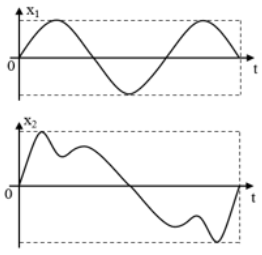
\includegraphics[scale=1.2]{../figs/VN12-2021-PH-TP015-1}
		\end{center}
		
		Chọn phát biểu đúng.
		\begin{mcq}(2)
			\item Độ cao của âm 1 lớn hơn âm 2.
			\item Hai âm có cùng âm sắc.
			\item Hai âm có cùng tần số.
			\item Độ cao của âm 2 lớn hơn âm 1.
		\end{mcq}
	}
	\loigiai{
		\textbf{Đáp án A.}
		
		Chu kì của âm 2 lớn hơn âm 1 nên tần số của âm 1 lớn hơn âm 2. Vậy độ cao của âm 1 lớn hơn âm 2.
	}
	
	\item \mkstar{2}
	
	\cauhoi{
		Dao động của sóng cơ tại một điểm trên mặt chất lỏng có phương trình là $u=A \cos (20x - 2000t)$, với $x$ đo bằng mét, $t$ đo bằng giây. Tốc độ truyền sóng trên mặt chất lỏng là
		
		\begin{mcq}(4)
			\item $\SI{200}{m/s}$.
			\item $\SI{20}{m/s}$.
			\item $\SI{100}{m/s}$.
			\item $\SI{10}{m/s}$.
		\end{mcq}
	}
	\loigiai{
		\textbf{Đáp án C.}
		
		Phương trình sóng tại một điểm có dạng tổng quát:
		$$u= A \cos \left(\omega t - \dfrac{2\pi d}{\lambda}\right)$$
		
		So sánh với phương trình $u=A \cos (20x - 2000 t) = A \cos (2000t - 20x)$, ta có:
		$$20=\dfrac{2\pi}{\lambda} \Rightarrow \lambda = \dfrac{\pi}{10}\ \text{m}.$$
		$$\omega = \SI{2000}{rad/s}.$$
		
		Vậy tốc độ truyền sóng là
		$$v=\lambda f = \lambda \dfrac{\omega}{2\pi} = \SI{100}{m/s}.$$
	}
	
	\item \mkstar{2}
	
	\cauhoi{
		Một sóng có tần số $\SI{100}{Hz}$ truyền trong một môi trường với tốc độ $\SI{50}{m/s}$. Bước sóng của sóng này là
		
		\begin{mcq}(4)
			\item $\SI{0.25}{m}$.
			\item $\SI{1.0}{m}$.
			\item $\SI{0.75}{m}$.
			\item $\SI{0.5}{m}$.
		\end{mcq}
	}
	\loigiai{
		\textbf{Đáp án D.}
		
		Bước sóng của sóng này là
		$$\lambda = \dfrac{v}{f} = \SI{0.5}{m}.$$
	}
	
	\item \mkstar{2}
	
	\cauhoi{
		Cho hai nguồn sóng kết hợp $\text{S}_1$, $\text{S}_2$ giống hệt nhau, cách nhau $\SI{5}{cm}$. Sóng do hai nguồn này tạo ra có bước sóng $\SI{2}{cm}$. Trên đoạn $\text{S}_1 \text{S}_2$ quan sát được số cực đại giao thoa là
		
		\begin{mcq}(4)
			\item 7.
			\item 5.
			\item 9.
			\item 3.
		\end{mcq}
	}
	\loigiai{
		\textbf{Đáp án B.}
		
		Điều kiện xảy ra cực đại giao thoa:
		$$- \dfrac{\text{S}_1 \text{S}_2}{\lambda} \leq k \leq \dfrac{\text{S}_1 \text{S}_2}{\lambda} \Rightarrow \SI{-2.5}{} \leq k \leq \SI{2.5}{}$$
		
		Vậy có 5 điểm thỏa mãn.
	}
	
	\item \mkstar{2}
	
	\cauhoi{
		Một sóng cơ học lan truyền dọc theo trục O$x$ có phương trình $u=12 \cos (20t - 4x)\ \text{cm}$, trong đó $x$ là tọa độ tính bằng mét, $t$ là thời gian được tính bằng giây. Tốc độ truyền sóng là
		
		\begin{mcq}(4)
			\item $\SI{5}{m/s}$.
			\item $\SI{0.5}{m/s}$.
			\item $\SI{40}{m/s}$.
			\item $\SI{4}{m/s}$.
		\end{mcq}
	}
	\loigiai{
		\textbf{Đáp án A.}
		
		Tần số sóng:
		$$f=\dfrac{\omega}{2\pi} = \xsi{\dfrac{10}{\pi}}{Hz}.$$
		
		Bước sóng:
		$$-\dfrac{2\pi}{\lambda} = -4 \Rightarrow \lambda = \dfrac{\pi}{2}\ \text{m}$$
		
		Tốc độ truyền sóng:
		$$v=\lambda f = \SI{5}{m/s}$$
	}
	
	\item \mkstar{2}
	
	\cauhoi{
		Một sóng có tần số $\SI{500}{Hz}$ lan truyền với tốc độ $\SI{350}{m/s}$. Hai điểm gần nhau nhất trên cùng một phương truyền sóng phải cách nhau một khoảng là bao nhiêu để chúng có độ lệch pha là $\dfrac{\pi}{3}\ \text{rad}$?
		
		\begin{mcq}(4)
			\item $\SI{4.285}{m}$.
			\item $\SI{0.233}{m}$.
			\item $\SI{0.476}{m}$.
			\item $\SI{0.116}{m}$.
		\end{mcq}
	}
	\loigiai{
		\textbf{Đáp án D.}
		
		Bước sóng:
		$$\lambda = \dfrac{v}{f} = \SI{0.7}{m}.$$
		
		Độ lệch pha:
		$$\Delta \varphi = \dfrac{2\pi}{\lambda} x = \dfrac{\pi}{3} \Rightarrow \dfrac{2}{\lambda} x = \dfrac{1}{3} \Rightarrow x = \SI{0.116}{m}.$$
	}
	
	\item \mkstar{2}
	
	\cauhoi{
		Một người quan sát trên mặt biển nhận thấy trong $\SI{4}{s}$ có 3 ngọn sóng biển đi qua trước mặt mình, khoảng cách giữa hai ngọn sóng liên tiếp là $\SI{12}{cm}$. Tốc độ truyền sóng trên mặt biển là
		
		\begin{mcq}(4)
			\item $\SI{24}{cm/s}$.
			\item $\SI{12}{cm/s}$.
			\item $\SI{6}{cm/s}$.
			\item $\SI{18}{cm/s}$.
		\end{mcq}
	}
	\loigiai{
		\textbf{Đáp án C.}
		
		Bước sóng: $\lambda = \SI{12}{cm}$.
		
		Chu kì: $2T = \SI{4}{s} \Rightarrow T = \SI{2}{s}$.
		
		Tốc độ truyền sóng:
		$$v=\dfrac{\lambda}{T} = \SI{6}{cm/s}.$$
	}
	
	\item \mkstar{2}
	
	\cauhoi{
		Người ta làm cho đầu O của một sợi dây căng ngang dao động điều hòa theo phương vuông góc với sợi dây, với chu kì $\SI{1.2}{s}$. Sau $\SI{3}{s}$, sóng truyền được $\SI{12}{m}$ theo chiều dài sợi dây. Bước sóng của sóng truyền trên dây là
		
		\begin{mcq}(4)
			\item $\SI{4}{m}$.
			\item $\SI{3.6}{m}$.
			\item $\SI{0.3}{m}$.
			\item $\SI{4.8}{m}$.
		\end{mcq}
	}
	\loigiai{
		\textbf{Đáp án D.}
		
		Vận tốc truyền sóng:
		$$v=\dfrac{s}{t} = \SI{4}{m/s}.$$
		
		Bước sóng:
		$$\lambda = vT = \SI{4.8}{m}.$$
	}
	
	\item \mkstar{2}
	
	\cauhoi{
		Hiệu số pha của hai sóng kết hợp, đồng pha truyền tới một điểm có giá trị nào sau đây để khi giao thoa, biên độ sóng có giá trị cực tiểu?
		
		\begin{mcq}(4)
			\item $\dfrac{\pi}{4}\ \text{rad}$.
			\item $\pi\ \text{rad}$.
			\item $\dfrac{\pi}{2}\ \text{rad}$.
			\item $0\ \text{rad}$.
		\end{mcq}
	}
	\loigiai{
		\textbf{Đáp án B.}
		
		Biên độ sóng khi giao thoa có giá trị cực tiểu khi $d_2 - d_1 = \xsi{\pi}{rad}$.
	}
	
	\item \mkstar{2}
	
	\cauhoi{
		Một sợi dây có chiều dài $l$ được giữ cố định ở hai đầu. Âm do dây phát ra có bước sóng lớn nhất bằng
		
		\begin{mcq}(4)
			\item $2l$.
			\item $\dfrac{l}{2}$.
			\item $l$.
			\item $\dfrac{l}{4}$.
		\end{mcq}
	}
	\loigiai{
		\textbf{Đáp án A.}
		
		Điều kiện xảy ra sóng dừng trên dây có hai đầu cố định:
		$$l=k \dfrac{\lambda}{2} \Rightarrow \lambda = \dfrac{2l}{k}.$$
		
		Bước sóng lớn nhất khi $k=1$, khi đó $\lambda = 2l$.
	}
	
	\item \mkstar{2}
	
	\cauhoi{
		Tại điểm O trên mặt nước có dao động điều hòa với chu kì $\SI{0.4}{s}$. Tốc độ truyền sóng trên mặt nước là $v=\SI{60}{cm/s}$. Khoảng cách từ đỉnh sóng thứ 2 đến đỉnh sóng thứ 6 kể từ O, trên cùng một phương chiều truyền sóng là
		
		\begin{mcq}(4)
			\item $\SI{96}{cm}$.
			\item $\SI{120}{cm}$.
			\item $\SI{24}{cm}$.
			\item $\SI{48}{cm}$.
		\end{mcq}
	}
	\loigiai{
		\textbf{Đáp án A.}
		
		Bước sóng:
		$$\lambda = vT = \SI{24}{cm}.$$
		
		Khoảng cách từ đỉnh sóng thứ 2 đến đỉnh sóng thứ 6: $4\lambda = \SI{96}{cm}$.
	}
	
	\item \mkstar{2}
	
	\cauhoi{
		Một nguồn đặt tại O phát ra sóng cơ có bước sóng bằng $\SI{10}{m}$ và biên độ $\SI{2}{cm}$. Chọn gốc thời gian là lúc nguồn ở vị trí cân bằng và bắt đầu chuyển động theo chiều dương. Biết tốc độ truyền sóng là $\SI{5}{m/s}$. Phương trình dao động tại một điểm M cách O một khoảng $\SI{2.5}{cm}$ theo phương truyền sóng là
		
		\begin{mcq}(2)
			\item $u_\text{M} = 2 \cos (\pi t + \pi)\ \text{cm}$.
			\item $u_\text{M} = 2 \cos \left(\pi t - \dfrac{\pi}{2}\right)\ \text{cm}$.
			\item $u_\text{M} = 2 \cos (2\pi t + \pi)\ \text{cm}$.
			\item $u_\text{M} = 2 \cos \left(2 \pi t - \dfrac{\pi}{2}\right)\ \text{cm}$.
		\end{mcq}
	}
	\loigiai{
		\textbf{Đáp án A.}
		
		Ta có: $\lambda = vT \Rightarrow T = \dfrac{\lambda}{v} = \SI{2}{s} \Rightarrow \omega = \dfrac{2\pi}{T} = \xsi{\pi}{rad/s}$.
		
		Phương trình sóng tại O:
		$$u_\text{O} = A \cos \left(\pi t - \dfrac{\pi}{2}\right)\ \text{cm}.$$
		
		Phương trình sóng tại M:
		$$u_\text{M} = A \cos (\pi t - \dfrac{\pi}{2} - \dfrac{2\pi d}{\lambda}).$$
		
		Mà $d=\SI{2.5}{m}$, suy ra: $\dfrac{2\pi d}{\lambda} = \dfrac{\pi}{2}\ \text{rad}$. Vậy:
		$$u_\text{M} = 2 \cos (\pi t + \pi)\ \text{cm}.$$
	}
	
	\item \mkstar{2}
	
	\cauhoi{
		Để đo độ sâu của vực sâu nhất thế giới (Mariana ở Thái Bình Dương), người ta dùng phương pháp định vị hồi âm bằng sóng siêu âm. Sau khi phát ra siêu âm hướng xuống biển thì sau $\SI{14.53}{s}$ người ta mới nhận được tín hiệu phản xạ của nó từ đáy biển. Vận tốc truyền âm của siêu âm trong nước biển là $\SI{1500}{m/s}$, trong không khí là $\SI{340}{m/s}$. Độ sâu của vực Mariana đo được là
		
		\begin{mcq}(4)
			\item $\SI{2470.1}{m}$.
			\item $\SI{4940.2}{m}$.
			\item $\SI{21795.5}{m}$.
			\item $\SI{10897.5}{m}$.
		\end{mcq}
	}
	\loigiai{
		\textbf{Đáp án D.}
		
		Vì sóng âm truyền từ mặt biển xuống đáy vực rồi phản xạ từ đáy vực lên mặt biển, nên quãng đường sóng truyền bằng 2 lần độ sâu vực:
		$$2d = vt \Rightarrow d = \SI{10897.5}{m}.$$
	}
	
	\item \mkstar{3}
	
	\cauhoi{
		Trên mặt thoáng của một chất lỏng, một mũi nhọn O chạm vào mặt nước dao động điều hòa với tần số $f$ tạo thành sóng trên mặt thoáng với bước sóng $\lambda$. Xét trên hai phương truyền sóng O$x$ và O$y$ vuông góc với nhau. Gọi A là điểm thuộc O$x$ cách O một đoạn $16 \lambda$ và B là điểm thuộc O$y$ cách O một đoạn $12\lambda$. Tìm số điểm dao động ngược pha với nguồn trên đoạn AB.
		
		\begin{mcq}(4)
			\item 8 điểm.
			\item 9 điểm.
			\item 6 điểm.
			\item 12 điểm.
		\end{mcq}
	}
	\loigiai{
		\textbf{Đáp án A.}
		
		Ta có: $\text{AB} = \sqrt{\text{OA}^2 + \text{OB}^2} = 20 \lambda$.
		
		Để một điểm ngược pha với nguồn thì $d=k \lambda$, với $k$ là số bán nguyên.
		
		Áp dụng hệ thức lượng, ta có $\text{OH} = \SI{9.6}{}\lambda$.
		\begin{center}
			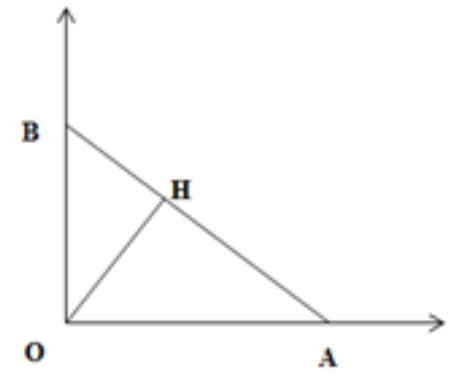
\includegraphics[scale=0.8]{../figs/VN12-2021-PH-TP015-5}
		\end{center}
	
		Số điểm nằm trên đoạn AH ngược pha với nguồn:
		$$\text{OH} \leq d \leq \text{OA} \Rightarrow k = \SI{10.5}{};\ \SI{11.5}{};\ \SI{12.5}{};\ \SI{13.5}{};\ \SI{14.5}{};\ \SI{15.5}{}.$$
		
		Số điểm nằm trên đoạn BH ngược pha với nguồn:
		$$\text{OH} \leq d \leq \text{OB} \Rightarrow k = \SI{10.5}{};\ \SI{11.5}{}.$$
		
		Vậy có tổng cộng 8 điểm thỏa mãn yêu cầu.
	}
	
	\item \mkstar{3}
	
	\cauhoi{
		Tại O có một nguồn phát sóng cơ với tần số $f=\SI{20}{Hz}$, tốc độ truyền sóng là $\SI{60}{cm/s}$. Ba điểm thẳng hàng A, B, C nằm trên cùng phương truyền sóng và cùng phía so với O. Biết $\text{OA} = \SI{8}{cm}$, $\text{OB} = \SI{25.5}{cm}$, $\text{OC} = \SI{40.5}{cm}$. Số điểm dao động cùng pha với A trên đoạn BC là
		
		\begin{mcq}(4)
			\item 3 điểm.
			\item 5 điểm.
			\item 4 điểm.
			\item 6 điểm.
		\end{mcq}
	}
	\loigiai{
		\textbf{Đáp án B.}
		
		Bước sóng:
		$$\lambda = \dfrac{v}{f} = \SI{3}{cm}.$$
		
		Để M nằm giữa BC và cùng pha với A thì:
		$$d_\text{M} - d_\text{A} = k\lambda \Rightarrow d_\text{M} = 8 + 3k\ (k \in \mathbb{Z}).$$
		
		Áp điều kiện:
		$$\SI{25.5}{cm} \leq 8 + 3k \leq \SI{40.5}{cm} \Rightarrow k = 6;\ 7;\ 8;\ 9;\ 10.$$
		
		Có 5 điểm thỏa mãn.
	}
	
	\item \mkstar{3}
	
	\cauhoi{
		Khi cường độ âm tăng gấp 1000 lần thì mức cường độ âm tăng
		
		\begin{mcq}(4)
			\item $\SI{1000}{dB}$.
			\item $\SI{20}{dB}$.
			\item $\SI{30}{dB}$.
			\item $\SI{40}{dB}$.
		\end{mcq}
	}
	\loigiai{
		\textbf{Đáp án C.}
		
		Công thức liên hệ giữa $L$ và $I$:
		$$L'-L = 10 \log \dfrac{I'}{I} = 10 \log 1000 = \SI{30}{dB}.$$
		
		Vậy mức cường độ âm tăng $\SI{30}{dB}$.
	}
	
	\item \mkstar{3}
	
	\cauhoi{
		Ở mặt thoáng của chất lỏng có hai nguồn sóng A, B cách nhau $\SI{18}{cm}$, dao động theo phương thẳng đứng với phương trình $u_\text{A} = u_\text{B} = a \cos (20\pi t)$ ($t$ tính bằng s). Tốc độ truyền sóng trên mặt chất lỏng là $\SI{50}{cm/s}$. Gọi M là điểm ở mặt chất lỏng gần A nhất sao cho phần tử chất lỏng tại M dao động với biên độ cực đại và cùng pha với nguồn A. Khoảng cách AM là
		
		\begin{mcq}(4)
			\item $\SI{2.5}{cm}$.
			\item $\SI{2.0}{cm}$.
			\item $\SI{5.0}{cm}$.
			\item $\SI{1.25}{cm}$.
		\end{mcq}
	}
	\loigiai{
		\textbf{Đáp án C.}
		
		Bước sóng là
		$$\lambda = \dfrac{v}{f} = \SI{5}{cm}.$$
		
		Áp dụng kết quả bài toán điều kiện để một vị trí cực đại và cùng pha với nguồn:
		$$
		\begin{cases}
			d_2 - d_1 = 2k \lambda \\
			d_2 + d_1 = 2m\lambda
		\end{cases}
	$$
	hoặc
	$$
		\begin{cases}
			d_2 - d_1 = (2k+1) \lambda \\
			d_2 + d_1 = (2m+1) \lambda
		\end{cases}
	$$
	$$
	\Rightarrow d_1 = (m-k) \lambda
		$$
		
		Do đó $d_\text{1 min}$ khi $(m-k)_\text{min} \Rightarrow d_\text{1 min} = \lambda = \SI{5}{cm}$.
	}
	
	\item \mkstar{3}
	
	\cauhoi{
		Một ống có một đầu bịt kín tạo ra âm cơ bản của nốt Đô có tần số $\SI{130.5}{Hz}$. Nếu người ta để hở đầu đó thì khi đó âm cơ bản tạo ra có tần số bằng bao nhiêu?
		
		\begin{mcq}(4)
			\item $\SI{522}{Hz}$.
			\item $\SI{491.5}{Hz}$.
			\item $\SI{261}{Hz}$.
			\item $\SI{195.25}{Hz}$.
		\end{mcq}
	}
	\loigiai{
		\textbf{Đáp án C.}
		
		Ống sao có một đầu bịt kín nên tần số để có sóng dừng trong ống là
		$$f=(2n+1) \dfrac{v}{4L} = (2n+1) f_\text{cb1}.$$
		
		Nếu để hở cả hai đầu thì điều kiện của tần số là
		$$f=n \dfrac{v}{2L} = n \cdot f_\text{cb2}.$$
		
		Ta thấy $f_\text{cb2} = 2 f_\text{cb1} = \SI{261}{Hz}$.
	}
	
	\item \mkstar{3}
	
	\cauhoi{
		Một sóng hình sin đang truyền trên một sợi dây, theo chiều dương của trục O$x$. Hình vẽ dưới đây mô tả hình dạng của sợi dây ở các thời điểm $t_1$ và $t_2=t_1+\SI{0.3}{s}$.
		\begin{center}
			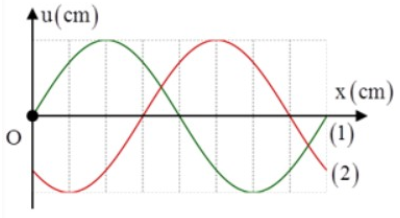
\includegraphics[scale=1]{../figs/VN12-2021-PH-TP015-2}
		\end{center}
		
		Chu kì của sóng là
		\begin{mcq}(4)
			\item $\SI{0.9}{s}$.
			\item $\SI{0.4}{s}$.
			\item $\SI{0.6}{s}$.
			\item $\SI{0.8}{s}$.
		\end{mcq}
	}
	\loigiai{
		\textbf{Đáp án D.}
		
		Từ đồ thị ta thấy trong khoảng thời gian $\Delta t = \SI{0.3}{s}$, đỉnh sóng đi được quãng đường $S=\SI{3}{cm}$.
		
		Vận tốc truyền sóng: $v=\dfrac{S}{\Delta t} = \SI{10}{cm/s}$.
		
		Bước sóng của sóng: $\lambda = \SI{8}{cm}$.
		
		Vậy chu kì của sóng là $T=\dfrac{\lambda}{v} = \SI{0.8}{s}$.
	}
	
	\item \mkstar{3}
	
	\cauhoi{
		Hai điểm A, B nằm trên cùng một đường thẳng đi qua một nguồn âm điểm phát ra âm đẳng hướng và ở hai phía so với nguồn âm. Biết mức cường độ âm tại A và tại trung điểm của AB lần lượt là $\SI{50}{dB}$ và $\SI{44}{dB}$. Mức cường độ âm tại B là
		
		\begin{mcq}(4)
			\item $\SI{28}{dB}$.
			\item $\SI{36}{dB}$.
			\item $\SI{38}{dB}$.
			\item $\SI{47}{dB}$.
		\end{mcq}
	}
	\loigiai{
		\textbf{Đáp án B.}
		
		Vì A, B nằm hai bên nguồn O nên $\text{OM} = \dfrac{\text{OB} - \text{OA}}{2}$.
		
		$$L_\text{A} - L_\text{M} = 20 \log \dfrac{\text{OM}}{\text{OA}} = 6 \Rightarrow \text{OM} = 2 \text{OA} \Rightarrow \text{OB} = 5 \text{OA}.$$
		
		$$L_\text{A} - L_\text{B} = 20 \log \dfrac{\text{OB}}{\text{OA}} = 20 \log 5 \Rightarrow L_\text{B} = 50 - 20 \log 5 = \SI{36}{dB}.$$
	}
	
	\item \mkstar{3}
	
	\cauhoi{
		Hai họa âm liên tiếp do một dây đàn phát ra có tần số hơn kém nhau $\SI{56}{Hz}$. Họa âm thứ ba và họa âm thứ năm có tần số lần lượt bằng bao nhiêu?
		
		\begin{mcq}(2)
			\item $\SI{162}{Hz}$ và $\SI{280}{Hz}$.
			\item $\SI{16}{Hz}$ và $\SI{28}{Hz}$.
			\item $\SI{12}{Hz}$ và $\SI{20}{Hz}$.
			\item $\SI{126}{Hz}$ và $\SI{208}{Hz}$.
		\end{mcq}
	}
	\loigiai{
		\textbf{Đáp án A.}
		
		Hai họa âm liên tiếp hơn kém nhau $\SI{56}{Hz}$ nên ta có:
		$$f_n - f_{n-1} = 56 \Leftrightarrow nf_1 - (n-1)f_1 = 56 \Rightarrow f_1 = \SI{56}{Hz}.$$
		
		Từ đó ta có tần số của họa âm thứ ba và thứ năm là
		$$f_3 = 3f_1 = \SI{162}{Hz}$$
		$$f_5 = 5f_1 = \SI{280}{Hz}$$
	}
	
	\item \mkstar{3}
	
	\cauhoi{
		Một sợi dây đàn hồi căng ngang, đang có sóng dừng ổn định. Khoảng thời gian giữa hai lần liên tiếp sợi dây duỗi thẳng là $\SI{0.1}{s}$. tốc độ truyền sóng trên dây là $\SI{3}{m/s}$. Khoảng cách giữa hai điểm gần nhau nhất trên sợi dây dao động cùng pha và có biên độ dao động bằng một nửa biên độ của bụng sóng là
		
		\begin{mcq}(4)
			\item $\SI{10}{cm}$.
			\item $\SI{8}{cm}$.
			\item $\SI{20}{cm}$.
			\item $\SI{30}{cm}$.
		\end{mcq}
	}
	\loigiai{
		\textbf{Đáp án C.}
		
		Khoảng thời gian giữa hai lần liên tiếp sợi dây duỗi thẳng là $\dfrac{T}{2} = \SI{0.1}{s}$, suy ra $T=\SI{0.2}{s}$. Suy ra bước sóng:
		$$\lambda = v T = \SI{0.6}{m}.$$
		
		Khoảng cách từ một điểm nút đến vị trí có biên độ bằng nửa biên độ cực đại là $\dfrac{\lambda}{2}$.
		
		Hai điểm gần nhau nhất trên sợi dây dao động cùng pha, suy ra 2 điểm đó cùng thuộc một bó sóng.
		
		Khoảng cách cần tìm:
		$$\dfrac{\lambda}{2} - \dfrac{\lambda}{12} - \dfrac{\lambda}{3} = \dfrac{\lambda}{3} = \SI{20}{cm}.$$
	}
	
	\item \mkstar{3}
	
	\cauhoi{
		Tại hai điểm A, B trên mặt chất lỏng cách nhau $\SI{15}{cm}$ có hai nguồn phát sóng kết hợp, dao động theo phương trình $u_1 = a \cos 40\pi t\ \text{cm}$ và $u_2 = b \cos (40\pi t + \pi)\ \text{cm}$. Tốc độ truyền sóng trên bề mặt chất lỏng là $\SI{40}{cm/s}$. Gọi E, F là hai điểm trên đoạn AB sao cho $\text{AE} = \text{EF} = \text{FB}$. Tìm số cực đại trên $\text{EF}$.
		
		\begin{mcq}(4)
			\item 5.
			\item 6.
			\item 4.
			\item 7.
		\end{mcq}
	}
	\loigiai{
		\textbf{Đáp án B.}
		
		Tại E ($d_1=\SI{5}{cm}$; $d_2 = \SI{10}{cm}$) suy ra $\Delta d_\text{E} = \SI{5}{cm}$.
		
		Tại F ($d_1=\SI{10}{cm}$; $d_2=\SI{5}{cm}$) suy ra $\Delta d_\text{F} = \SI{-5}{cm}$.
		
		$$\lambda = \dfrac{v}{f} = \SI{2}{cm}.$$
		
		Vì 2 nguồn dao động ngược pha: $\Delta \varphi = \xsi{\pi}{rad}$.
		
		Số cực đại:
		$$\dfrac{\Delta d_\text{F}}{\lambda} - \dfrac{\Delta \varphi}{2\pi} \leq k \leq \dfrac{\Delta d_\text{E}}{\lambda} - \dfrac{\Delta \varphi}{2\pi} \Rightarrow -3 \leq k \leq 2.$$
		
		Có 6 điểm dao động cực đại.
	}
	
	\item \mkstar{3}
	
	\cauhoi{
		Thực hiện thí nghiệm giao thoa sóng cơ trên mặt chất lỏng với hai nguồn cùng pha có cùng tần số $f=\SI{30}{Hz}$, vận tốc truyền sóng trong môi trường là $\SI{150}{cm/s}$. Trên mặt chất lỏng có 4 điểm có tọa độ lần lượt như sau: M ($d_1=\SI{25}{cm};\ d_2 = \SI{30}{cm}$); N ($d_1=\SI{5}{cm};\ d_2=\SI{10}{cm}$); O ($d_1 = \SI{7}{cm};\ d_2=\SI{12}{cm}$); P ($d_1 = \SI{27.5}{cm};\ d_2=\SI{30}{cm}$). Hỏi có mấy điểm nằm trên đường cực đại số 1?
		
		\begin{mcq}(4)
			\item 1.
			\item 2.
			\item 3.
			\item 4.
		\end{mcq}
	}
	\loigiai{
		\textbf{Đáp án C.}
		
		Ta có $\lambda = \dfrac{v}{f} = \SI{5}{cm}$.
		
		Tại M: $\Delta d= d_2 - d_1 = \SI{5}{cm} = \lambda \Rightarrow$ nằm trên đường cực đại số 1.
		
		Tại N: $\Delta d= d_2 - d_1 = \SI{5}{cm} = \lambda \Rightarrow$ nằm trên đường cực đại số 1.
		
		Tại O: $\Delta d= d_2 - d_1 = \SI{5}{cm} = \lambda \Rightarrow$ nằm trên đường cực đại số 1.
		
		Tại P: $\Delta d= d_2 - d_1 = \SI{2.5}{cm} = \dfrac{\lambda}{2} \Rightarrow$ nằm trên đường cực tiểu số 1.
		
		Có 3 điểm M, N, O nằm trên đường cực đại số 1.
	}
	
	\item \mkstar{3}
	
	\cauhoi{
		Ở mặt nước có hai nguồn kết hợp đặt tại hai điểm A và B, dao động cùng pha theo phương thẳng đứng, phát ra hai sóng có bước sóng $\lambda$. Trên AB có 9 vị trí mà ở đó các phần tử nước dao động với biên độ cực đại. Gọi C và D là hai điểm ở mặt nước sao cho ABCD tạo thành hình vuông. Gọi M là một điểm thuộc cạnh CD và nằm trên vân cực đại giao thoa bậc nhất ($\text{MA} - \text{MB} = \lambda$). Biết phần tử tại M dao động cùng pha với các nguồn. Độ dài đoạn AB \textbf{gần nhất} với giá trị nào sau đây?
		
		\begin{mcq}(4)
			\item $\SI{4.6}{\lambda}$.
			\item $\SI{4.8}{\lambda}$.
			\item $\SI{4.4}{\lambda}$.
			\item $\SI{4.7}{\lambda}$.
		\end{mcq}
	}
	\loigiai{
		\textbf{Đáp án B.}
		
		\begin{center}
			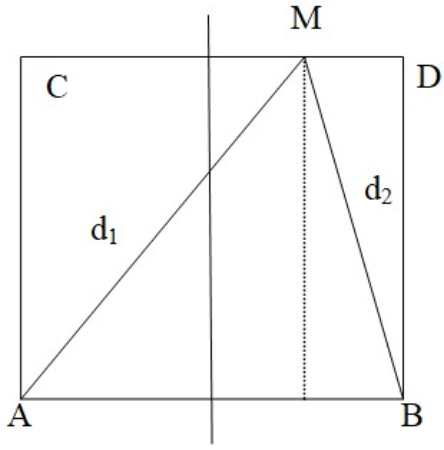
\includegraphics[scale=0.8]{../figs/VN12-2021-PH-TP015-6}
		\end{center}
	
		M là cực đại giao thoa và cùng pha với hai nguồn nên $d_1 - d_2 = n \lambda$, $d_1 + d_2 = m \lambda$, với $n$, $m$ là số nguyên cùng lẻ hoặc cùng chẵn.
		
		Vì $n=1 \Rightarrow m$ là số lẻ.
		
		Ta có: $d_1 + d_2 > \text{AB}$, $4\lambda \leq \text{AB} \leq 5 \lambda$.
		
		Từ các phương trình trên, ta có: $d_1 - d_2 = \lambda$, $d_1 + d_2 = 11 \lambda$.
		
		Suy ra: $d_1 = 6 \lambda$, $d_2 = 5 \lambda$.
		
		Ta có: $\sqrt{(6\lambda)^2 - \text{AB}^2} + \sqrt{(5 \lambda)^2 - \text{AB}^2} = \text{AB}^2 \Rightarrow \text{AB} = \SI{4.8336}{\lambda}$.
	}
	
	\item \mkstar{3}
	
	\cauhoi{
		Hai nguồn sóng kết hợp $\text{S}_1$ và $\text{S}_2$ nằm trên mặt chất lỏng, thực hiện các dao động điều hòa theo phương vuông góc với mặt chất lỏng với hiệu số pha ban đầu bằng $\varphi$. Biết rằng trên đường nối hai nguồn, trong số những điểm có biên độ dao động bằng 0 thì điểm M gần đường trung trực nhất cách đường trung trực một khoảng bằng $\lambda /6$. Hiệu số pha ban đầu $\varphi$ có giá trị bằng
		
		\begin{mcq}(4)
			\item $\dfrac{2\pi}{3}\ \text{rad}$.
			\item $\dfrac{\pi}{2}\ \text{rad}$.
			\item $\dfrac{\pi}{3}\ \text{rad}$.
			\item $\dfrac{\pi}{6}\ \text{rad}$.
		\end{mcq}
	}
	\loigiai{
		\textbf{Đáp án C.}
		
		Điểm cực tiểu (là điểm M) trên $\text{S}_1 \text{S}_2$ nằm gần điểm cực đại trung tâm nhất (là điểm O) cách O một khoảng bằng $\lambda / 4$. Gọi trung điểm của $\text{S}_1 \text{S}_2$ là I.
		
		TH1: điểm M nằm giữa I và O. Ta có $\text{IM} + \text{MO} = \text{IO}$, suy ra:
		$$\dfrac{\lambda}{6} + \dfrac{\lambda}{4} = \dfrac{\Delta \varphi \lambda}{4\pi} \Rightarrow \Delta \varphi = \xsi{\dfrac{5\pi}{3}}{rad}.$$
		
		TH2: điểm I nằm giữa M và O. Ta có $\text{IM} + \text{IO} = \text{MO}$, suy ra:
		$$\dfrac{\lambda}{6} + \dfrac{\Delta \varphi \lambda}{4\pi} = \dfrac{\lambda}{4} \Rightarrow \Delta \varphi = \xsi{\dfrac{\pi}{3}}{rad}.$$
	}
	
	\item \mkstar{3}
	
	\cauhoi{
		Hai nguồn âm nhỏ giống nhau phát ra âm thanh cùng pha, cùng biên độ và cùng tần số tại A và B. Tai của một người ở điểm N với $\text{AN} = \SI{2}{m}$ và $\text{BN} = \SI{1.625}{m}$. Tốc độ truyền âm trong không khí là $\SI{330}{m/s}$. Bước sóng dài nhất để người này không nghe được âm thanh từ hai nguồn phát ra là
		
		\begin{mcq}(4)
			\item $\SI{0.375}{m}$.
			\item $\SI{0.75}{m}$.
			\item $\SI{0.50}{m}$.
			\item $\SI{0.25}{m}$.
		\end{mcq}
	}
	\loigiai{
		\textbf{Đáp án B.}
		
		Để tai người này không nghe được âm thì tai đặt ở vị trí cực tiểu giao thoa:
		$$\text{AN} - \text{BN} = \left(k + \dfrac{1}{2}\right) \lambda \Rightarrow \lambda = \dfrac{\text{AN} - \text{BN}}{k + \SI{0.5}{}}.$$
		
		Bước sóng lớn nhất ứng với $k=0$, khi đó:
		$$\lambda = \dfrac{\text{AN} - \text{BN}}{\SI{0.5}{}} = \SI{0.75}{m}.$$
	}
	
	\item \mkstar{3}
	
	\cauhoi{
		Trong giờ thực hành hiện tượng sóng dừng trên dây, một học sinh thực hiện như sau: tăng dần tần số của máy phát dao động thì thấy rằng khi sóng dừng xuất hiện trên dây tương ứng với 1 bó sóng và 9 bó sóng thì tần số thu được thỏa mãn $f_9 - f_1 = \SI{200}{Hz}$. Khi trên dây xuất hiện sóng dừng với 6 nút sóng thì máy phát tần số ở giá trị là
		
		\begin{mcq}(4)
			\item $\SI{150}{Hz}$.
			\item $\SI{125}{Hz}$.
			\item $\SI{100}{Hz}$.
			\item $\SI{120}{Hz}$.
		\end{mcq}
	}
	\loigiai{
		\textbf{Đáp án B.}
		
		Với sóng dừng trên dây có hai đầu cố định thì chiều dài sợi dây phải thỏa:
		$$l=k \dfrac{v}{2f} \Rightarrow f =\dfrac{kv}{2l}.$$
		
		Với $f_9 - f_1 = \SI{200}{Hz}$, ta được:
		$$\dfrac{9v}{2l} - \dfrac{v}{2l} = \dfrac{8v}{2l} = \SI{200}{Hz} \Rightarrow \dfrac{v}{2l} = \dfrac{200}{8}.$$
		
		Với 6 nút sóng thì có 5 bó sóng, thay $k=5$ ta được $f_5$ là
		$$f_5 = \dfrac{5v}{2l} = \SI{125}{Hz}.$$
	}
	
	\item \mkstar{4}
	
	\cauhoi{
		Sóng ngang có tần số $f$ truyền trên một sợi dây đàn hồi rất dài với tốc độ $\SI{4.5}{m/s}$. Xét hai điểm M và N trên cùng một phương truyền sóng, cách nhau một khoảng $x$ nhỏ hơn bước sóng. Sóng truyền từ N đến M. Đồ thị biểu diễn li độ sóng của M và N theo thời gian như hình dưới.
		\begin{center}
			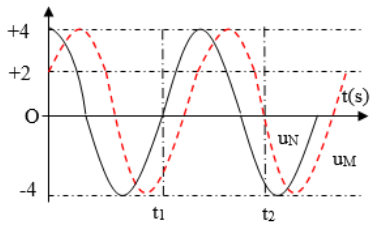
\includegraphics[scale=1]{../figs/VN12-2021-PH-TP015-3}
		\end{center}
		
		Biết $t_1 = \SI{0.05}{s}$. Tại thời điểm $t_2$, khoảng cách giữa phần tử chất lỏng tại M và N có giá trị \textbf{gần nhất} với giá trị nào sau đây?
		\begin{mcq}(4)
			\item $\SI{4.8}{cm}$.
			\item $\SI{6.2}{cm}$.
			\item $\SI{5.7}{cm}$.
			\item $\SI{3.5}{cm}$.
		\end{mcq}
	}
	\loigiai{
		\textbf{Đáp án B.}
		
		Từ đồ thị ta thấy đường N (màu đen) sớm pha hơn M (màu đỏ) một góc là $\Delta \varphi = \xsi{\dfrac{\pi}{3}}{rad}$.
		
		Do đó khoảng cách MN theo phương truyền sóng là $\text{MN} = \dfrac{\lambda}{6}$.
		
		Dựa vào đường màu đen, ta xác định được khoảng thời gian từ $t=0$ đến $t=t_1 = \SI{0.05}{s}$ là $\dfrac{T}{4} + \dfrac{T}{2} = \dfrac{3T}{4}$. Suy ra $T=\xsi{\dfrac{1}{15}}{s}$.
		
		Tính được $\lambda = vT = \SI{30}{cm}$ và $\text{MN} = \SI{5}{cm}$.
		
		Viết phương trình dao động của M và N, ta được:
		$$u_\text{M}=4 \cos \left(30\pi t - \dfrac{\pi}{3}\right)\ \text{cm}.$$
		$$u_\text{N} = 4 \cos (30\pi t)\ \text{cm}.$$
		
		Dựa vào đồ thị thì ta thấy $t_2 = t_1 + \dfrac{T}{2} + \dfrac{T}{6} $, ta xác định được:
		$$|u_\text{M} - u_\text{N}|_{t_2} = \xsi{2\sqrt{3}}{cm}.$$
		$$\Rightarrow \text{MN}_{t_2} = \sqrt{5^2 + 2^2 \cdot 3} = \SI{6.083}{cm}.$$
		
		Vậy $\SI{6.2}{cm}$ là đáp án gần đúng nhất.
	}
	
	\item \mkstar{4}
	
	\cauhoi{
		Một sợi dây đàn hồi căng ngang, đang có sóng dừng ổn định. Trên dây, A là điểm nút, còn B là điểm bụng ở gần A nhất, còn C là trung điểm của AB. Cho $\text{AB} = \SI{10}{cm}$. Biết khoảng thời gian ngắn nhất giữa hai lần mà li độ dao động của phần tử tại B bằng biên độ dao động của phần tử tại C là $\SI{0.2}{s}$. Tốc độ truyền sóng trên dây là
		
		\begin{mcq}(4)
			\item $\SI{2}{m/s}$.
			\item $\SI{0.5}{m/s}$.
			\item $\SI{1}{m/s}$.
			\item $\SI{0.25}{m/s}$.
		\end{mcq}
	}
	\loigiai{
		\textbf{Đáp án B.}
		
		Vì B là điểm bụng gần nút A nhất nên:
		$$\text{AB} = \SI{10}{cm} = \dfrac{\lambda}{4} \Rightarrow \lambda = \SI{40}{cm}.$$
		
		Tại C thì $x=\dfrac{\lambda}{8} = \SI{5}{cm}$. Biên độ dao động của C là
		$$A_\text{C} = 2A \sin \left(\dfrac{2\pi \lambda}{8\lambda}\right) = A\sqrt{2}.$$
		
		Tương tự, biên độ dao động tại B là $2A$.
		
		\begin{center}
			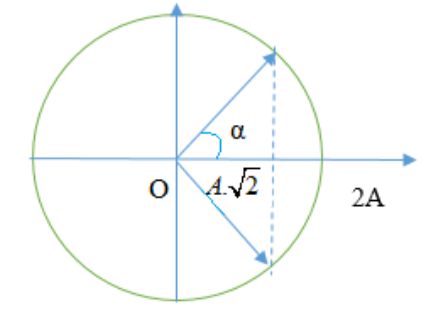
\includegraphics[scale=1]{../figs/VN12-2021-PH-TP015-7}
		\end{center}
	
		Dựa đồ giản đồ vectơ quay, ta có độ lớn góc $\alpha$ là
		$$\alpha = \arccos \dfrac{A \sqrt{2}}{2A} = 45^\circ.$$
		
		Vậy thời gian giữa hai lần liên tiếp B có li độ bằng biên độ của C là
		$$t = \dfrac{2 \cdot 45^\circ}{360^\circ} \cdot T = \dfrac{T}{4}.$$
		
		Vậy chu kì dao động là $T=4t=\SI{0.8}{s}$, vận tốc truyền sóng là $v=\dfrac{\lambda}{T} = \SI{50}{cm}$.
	}
	
	\item \mkstar{4}
	
	\cauhoi{
		Trên một sợi dây dài đang có sóng ngang truyền qua, hình dạng của một đoạn dây tại hai thời điểm $t_1$ và $t_2$ được cho như hình dưới.
		\begin{center}
			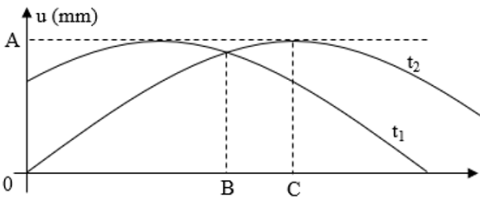
\includegraphics[scale=1]{../figs/VN12-2021-PH-TP015-4}
		\end{center}
	
		Li độ của các phần tử tại B và C ở thời điểm $t_1$ lần lượt là $\xsi{10\sqrt{3}}{mm}$ và $\SI{10}{mm}$. Biết $\Delta t = t_2 - t_1 = \xsi{\dfrac{\SI{0.05}{}}{6}}{s}$ và nhỏ hơn một chu kì sóng. Tốc độ dao động cực đại của các phần tử trên dây bằng
		\begin{mcq}(4)
			\item $\xsi{0,4\pi \sqrt{2}}{m/s}$.
			\item $\xsi{0,4\pi}{m/s}$.
			\item $\xsi{0,8\pi}{m/s}$.
			\item $\xsi{0,8\pi \sqrt{3}}{m/s}$.
		\end{mcq}
	}
	\loigiai{
		\textbf{Đáp án C.}
		
		Từ đồ thị, xác định được các điểm B, C tại thời điểm $t_1$, $t_2$ trên vòng tròn lượng giác:
		\begin{center}
			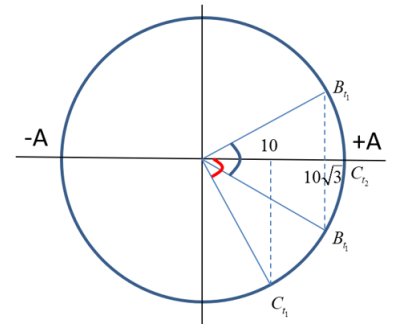
\includegraphics[scale=1]{../figs/VN12-2021-PH-TP015-8}
		\end{center}
	
	Ta có:
	$$\Delta \varphi_{\text C(t_1 \rightarrow t_2)} = \Delta \varphi_{\text B (t_1 \rightarrow t_2)} = \alpha = \omega \Delta t.$$
	
	Từ vòng tròn lượng giác, ta có $\cos \alpha = \dfrac{10}{A}$ và $\cos \dfrac{\alpha}{2} = \dfrac{10\sqrt{3}}{A}$.
	
	Suy ra $\cos \alpha = \dfrac{1}{2} \Rightarrow \alpha = 60^\circ \Rightarrow A = \SI{20}{mm}$.
	
	Mà $\alpha = \omega\Delta t \Rightarrow \omega = \dfrac{\alpha}{\Delta t} = \xsi{40\pi}{rad/s}$.
	
	Tốc độ cực đại:
	$$v_\text{max} = \omega A = \xsi{0,8\pi}{m/s}.$$
	}
	
	\item \mkstar{4}
	
	\cauhoi{
		Một sợi dây đang có sóng dừng ổn định. Sóng truyền trên dây có tần số $\SI{10}{Hz}$ và bước sóng $\SI{6}{cm}$. Trên dây, hai phần tử M và N có vị trí cân bằng cách nhau $\SI{8}{cm}$, M thuộc một bụng sóng dao động điều hòa với biên độ $\SI{6}{mm}$. Lấy $\pi^2 = 10$. Tại thời điểm $t$, phần tử M đang chuyển động với tốc độ $\xsi{6\pi}{cm/s}$ thì phần tử N chuyển động với gia tốc có độ lớn là
		
		\begin{mcq}(4)
			\item $\xsi{6\sqrt{3}}{m/s^2}$.
			\item $\SI{6}{m/s^2}$.
			\item $\xsi{6\sqrt{2}}{m/s^2}$.
			\item $\SI{3}{m/s^2}$.
		\end{mcq}
	}
	\loigiai{
		\textbf{Đáp án A.}
		
		Tần số góc của dao động là
		$$\omega = 2\pi f = 2\pi \cdot \SI{10}{Hz} = \xsi{20\pi}{rad/s}.$$
		
		Biên độ dao động của N là
		$$A_\text{N} = A_\text b \left|\cos \left(\dfrac{2\pi d}{\lambda}\right)\right| = \SI{0.006}{m} \cdot \left|\cos \left(\dfrac{2\pi \cdot \SI{0.08}{m}}{\SI{0.06}{m}}\right)\right| = \SI{0.003}{m}.$$
		
		Tại thời điểm M chuyển động với tốc độ $\xsi{6\pi}{cm/s}$ thì nó có li độ là
		$$\left(\dfrac{x_\text{M}}{A_\text{M}}\right)^2 + \left(\dfrac{v_\text{M}}{v_\text{M max}}\right)^2 = 1 \Rightarrow \left(\dfrac{x}{\SI{0.006}{m}}\right)^2 + \left(\dfrac{6\pi \cdot 10^{-2}\ \text{m/s}}{20\pi\ \text{rad/s} \cdot \SI{0.006}{m}}\right)^2 = 1 \Rightarrow x_\text{M} = \xsi{\dfrac{3\sqrt{3}}{1000}}{m}.$$
		
		Gia tốc của điểm N có thể suy ra bằng cách lập tỉ số giữa gia tốc của M và gia tốc của N:
		$$\left|\dfrac{a_\text{N}}{a_\text{M}}\right| = \left|\dfrac{a_\text{N}}{\omega^2 x_\text{M}}\right| = \dfrac{A_\text{N}}{A_\text{M}} \Rightarrow \left|\dfrac{a_\text{N}}{(20\pi\ \text{rad/s})^2 \cdot \xsi{\dfrac{3\sqrt{3}}{1000}}{m}}\right| = \dfrac{\SI{0.003}{m}}{\SI{0.006}{m}} \Rightarrow |a_\text{N}| = \xsi{6\sqrt{3}}{m/s^2}.$$
	}
	
	\item \mkstar{4}
	
	\cauhoi{
		Tại hai điểm A, B trên mặt nước cách nhau $\SI{16}{cm}$ có hai nguồn phát sóng giống nhau. Điểm M nằm trên mặt nước và trên đường trung trực của AB, cách trung điểm I của AB một khoảng nhỏ nhất bằng $\xsi{5\sqrt{5}}{cm}$ và luôn dao động cùng pha với I. Hỏi điểm N nằm trên mặt nước và nằm trên đường thẳng vuông góc với AB tại A, cách A một khoảng nhỏ nhất bằng bao nhiêu để N dao động với biên độ cực tiểu?
		\begin{mcq}(4)
			\item $\SI{9.22}{cm}$.
			\item $\SI{8.75}{cm}$.
			\item $\SI{2.14}{cm}$.
			\item $\SI{8.57}{cm}$.
		\end{mcq}
	}
	\loigiai{
		\textbf{Đáp án C.}
		
		\begin{center}
			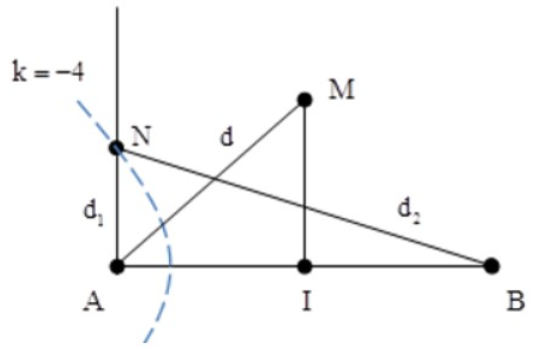
\includegraphics[scale=0.8]{../figs/VN12-2021-PH-TP015-9}
		\end{center}
	
		Vì hai nguồn đồng pha, M, I đều thuộc trung trực của AB nên để M và I dao động cùng pha thì:
		$$\text{MA} - \text{IA} = k \lambda.$$
		
		Mà M gần I nhất nên chọn $k=1$, do đó:
		$$\text{MA} = d_\text{A} = \SI{0.5}{}\text{AB} + \lambda = 8 + \lambda.$$
		
		Mặt khác $\text{MI} = \xsi{4\sqrt{5}}{cm}$ nên
		$$\text{MA} = \xsi{4\sqrt{5}}{cm} \Rightarrow \text{MA} = 8 + \lambda = \sqrt{\left(\dfrac{\text{AB}}{2}\right)^2 + \text{IM}^2} = 12 \Rightarrow \lambda = \SI{4}{cm}.$$
		
		Số điểm dao động với biên độ cực tiểu trên AB:
		$$-\dfrac{\text{AB}}{2} - \dfrac{1}{2} < k < \dfrac{\text{AB}}{2} - \dfrac{1}{2} \Rightarrow \SI{-4.5}{} < k < \SI{3.5}{}.$$
		
		Để N là một điểm cực tiểu và gần A nhất thì N phải nằm trên hyperbol cực tiểu có $k=\SI{-4}{}$. Vậy:
		$$
		\begin{cases}
			d_\text{1N} - d_\text{2N} = \SI{-3.5}{\lambda}\\
			d_\text{2N}^2 = d_\text{1N}^2 + \text{AB}^2
		\end{cases}
	\Rightarrow d_\text{1N} = \SI{2.14}{cm}.
		$$
	}
\end{enumerate}
\loigiai{\textbf{Đáp án}
	\begin{center}
		\begin{tabular}{|m{2.8em}|m{2.8em}|m{2.8em}|m{2.8em}|m{2.8em}|m{2.8em}|m{2.8em}|m{2.8em}|m{2.8em}|m{2.8em}|}
			\hline
			1. B & 2. B & 3. D & 4. A & 5. A & 6. B & 7. C & 8. A & 9. C & 10. D \\
			\hline
			11. B & 12. A & 13. D & 14. C & 15. D & 16. B & 17. A & 18. A & 19. A & 20. D\\
			\hline
			21. A & 22. B & 23. C & 24. C & 25. C & 26. D & 27. B & 28. A & 29. C & 30. B\\
			\hline
			31. C & 32. B & 33. C & 34. B & 35. B & 36. B & 37. B & 38. C & 39. A & 40. C\\
			\hline
		\end{tabular}
\end{center}}